\documentclass[tikz,border=2pt]{standalone}
\usepackage{amsmath,amssymb}
\usepackage{tikz}

\begin{document}
% The three axioms as areas: probabilities are nonnegative, the whole sample space has
% probability 1, and disjoint pieces add.
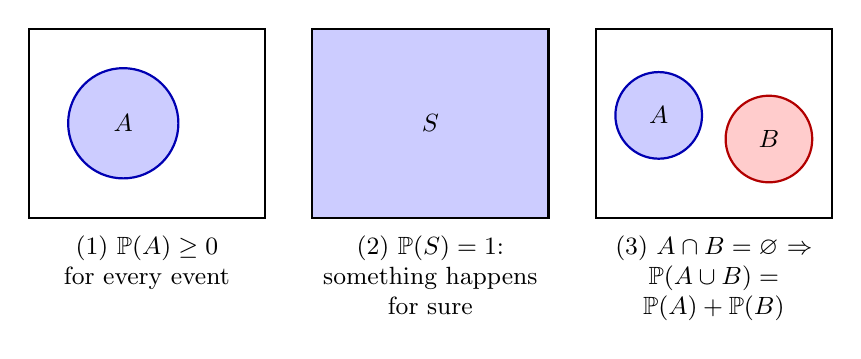
\begin{tikzpicture}[every node/.style={font=\small}]
	\begin{scope}
		\draw[thick] (-1.5,-1.2) rectangle (1.5,1.2);
		\fill[blue!20] (-0.3,0) circle (0.7);
		\draw[thick, blue!70!black] (-0.3,0) circle (0.7);
		\node at (-0.3,0) {$A$};
		\node[anchor=north, align=center] at (0,-1.3) {(1) $\mathbb{P}(A)\ge0$\\ for every event};
	\end{scope}
	\begin{scope}[xshift=3.6cm]
		\fill[blue!20] (-1.5,-1.2) rectangle (1.5,1.2);
		\draw[thick] (-1.5,-1.2) rectangle (1.5,1.2);
		\node at (0,0) {$S$};
		\node[anchor=north, align=center] at (0,-1.3) {(2) $\mathbb{P}(S)=1$:\\ something happens\\ for sure};
	\end{scope}
	\begin{scope}[xshift=7.2cm]
		\draw[thick] (-1.5,-1.2) rectangle (1.5,1.2);
		\fill[blue!20] (-0.7,0.1) circle (0.55);
		\fill[red!20] (0.7,-0.2) circle (0.55);
		\draw[thick, blue!70!black] (-0.7,0.1) circle (0.55);
		\draw[thick, red!70!black] (0.7,-0.2) circle (0.55);
		\node at (-0.7,0.1) {$A$};
		\node at (0.7,-0.2) {$B$};
		\node[anchor=north, align=center] at (0,-1.3) {(3) $A\cap B=\varnothing$ $\Rightarrow$\\ $\mathbb{P}(A\cup B)=$\\ $\mathbb{P}(A)+\mathbb{P}(B)$};
	\end{scope}
	
\end{tikzpicture}
\end{document}
